% !TeX spellcheck = it_IT
\section{Statistica descrittiva}
La statistica si occupa dello studio dei dati, ovvero della sua \textbf{raccolta}, \textbf{analisi} ed \textbf{interpretazione}. Le risposte dipendono dai dati e dalla conoscenza pregressa del problema, quindi da eventuali ipotesi ed assunzioni.\\
\begin{itemize}
	\item Statistica \textbf{descrittiva}: quando i dati vengono analizzati senza fare assunzioni esterne per evidenziarne la struttura e rappresentarli in modo efficace
	\item \textbf{Inferenza statistica}: studia i dati utilizzando un modello probabilistico, ovvero supponendo che i dati siano valori assunti da \textit{variabili aleatorie} con una certa \textit{distribuzione di probabilità} dipendente da parametri non noti che devono essere stimati. Il modello potrà poi fare previsioni.
\end{itemize}

\subsubsection{Campioni statistici}
\begin{definition}[Popolazione o Universo]
	Insieme di oggetti o fenomeni che si vuole studiare. Può essere \textbf{ideale}, ovvero tutti i possibili esiti, o \textbf{reale}.
\end{definition}
\begin{definition}[Carattere]
	Caratteristica degli individui della popolazione, ottenuta con la stessa procedura. Può essere:
	\begin{itemize}
		\item \textbf{Quantitativo} se gli esiti sono sumeri paragonabili tra loro
		\item \textbf{Qualitativo} altrimenti
	\end{itemize}
\end{definition}
\begin{definition}[Modalità]
	Uno dei possibili valori o attributi che può assumere il carattere. Se il carattere è quantitativo, si usa il termine \textbf{valore}.
\end{definition}
\begin{definition}[Campione statistico]
	Un sottoinsieme della popolazione scelto per rappresentarla.
\end{definition}
\begin{definition}[Dati]
	Gli esiti delle misure dei caratteri considerati sugli elementi del campione.
\end{definition}

\begin{observation}[Campione rappresentativo]
	Il problema di quando un campione sia o meno rappresentativo di tutta la popolazione è complesso e, in un certo senso, dà origine alla seguente distinzione:
	\begin{itemize}
		\item Statistica \textbf{descrittiva} o \textbf{deduttiva}: analizza il gruppo senza trarre alcuna conclusione su quello più grande
		\item Statistica \textbf{induttiva} o \textbf{referenziale}: dato un campione cerca di trarre conclusioni circa la popolazione. Queste sono valide se e solo se il campione è veramente significativo. Non ci sono certezze e le conclusioni sono rappresentate nel linguaggio della \textbf{probabilità}.
	\end{itemize}
\end{observation}
\begin{definition}[Frequenza di una modalità]
	Può essere:
	\begin{itemize}
		\item \textbf{Assoluta}: il numero di volte in cui la modalità compare nei dati
		\item \textbf{Relativa}: frazione di volte in cui la modalità compare sul totale dei dati
	\end{itemize}
\end{definition}

\subsection{Rappresentazione grafica}
La rappresentazione grafica dei dati di un campione dipende dalla natura del carattere:
\begin{itemize}
	\item \textbf{Discreto}: se può assumere una quantità finita e relativamente piccola di modalità o valori
	\item \textbf{Continuo}: se può assumere un grande numero di dati
\end{itemize}

\subsubsection{Diagramma a barre}
Permette di rappresentare caratteri discreti.
\begin{center}
	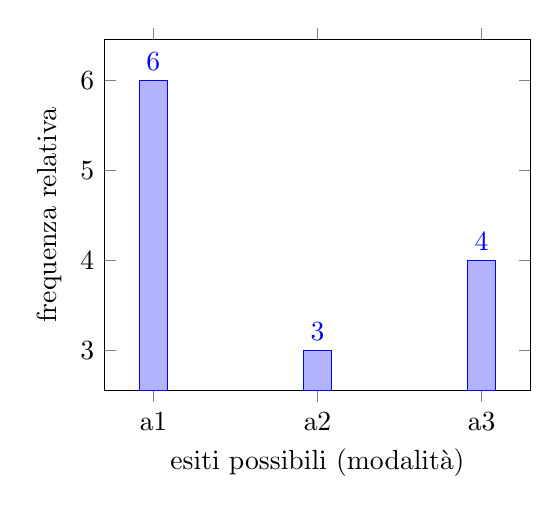
\begin{tikzpicture}
		\begin{axis}[
			width=7cm,
			ybar,
			enlargelimits=0.15,
			legend style={at={(0.5,-0.15)},
				anchor=north,legend columns=-1},
			ylabel={frequenza relativa},
			xlabel={esiti possibili (modalità)},
			symbolic x coords={a1,a2,a3},
			xtick=data,
			nodes near coords,
			nodes near coords align={vertical},
			]
			\addplot coordinates {(a1,6) (a2,3) (a3,4)};
		\end{axis}
	\end{tikzpicture}
\end{center}

\subsubsection{Diagramma a torta}
Sempre per rappresentare caratteri discreti, specialmente se le modalità sono poche.
\begin{center}
	\begin{tikzpicture}
		\pie{10/A, 20/B, 30/C, 40/D}
	\end{tikzpicture}
\end{center}

\subsubsection{Istogramma}
Consiste in una serie di colonne ognuna delle quali ha per base un intervallo numerico e per area la frequenza relativa dei dati contenuti nell'intervallo.

\begin{center}
	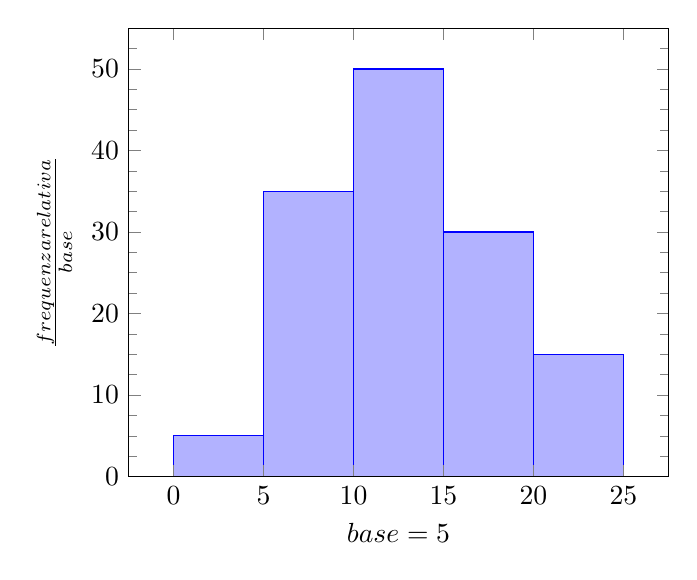
\begin{tikzpicture}
		\begin{axis}[
			ylabel={$\frac{\text{frequenza relativa}}{\text{base}}$},
			xlabel={$\text{base}=5$},
			ymin=0, ymax=55,
			minor y tick num = 3,
			area style,
			]
			\addplot+[ybar interval,mark=no] plot coordinates { (0, 5) (5, 35) (10, 50) (15, 30) (20, 15) (25, 0) };
		\end{axis}
	\end{tikzpicture}
	$\text{Area}=\frac{\text{frequenza assoluta}}{\text{totale}} = b \cdot h$
\end{center}

\begin{observation}
	In alcuni libri di testo si prende come \textit{altezza}, invece che come area, la frequenza relativa dei dati nell'intervallo considerato. Se la base è uguale per tutti i rettangoli, ovvero tutti gli intervalli hanno la stessa ampiezza, la rappresentazione va comunque bene. Il problema nasce quando vogliamo utilizzare intervalli con ampiezze diverse.
\end{observation}

\begin{observation}
	La scelta delle ampiezze degli intervalli di base è cruciale. L'idea è di cercare un compromesso che ci permetta di non perdere troppe informazioni (ampiezza troppo grande) senza però rendere l'istogramma troppo dipendente da piccole variazioni (troppi intervalli).
\end{observation}

\paragraph{Forme} Un istogramma può avere varie forme:
\begin{itemize}
	\item \textbf{Normale} se ha la forma di una \textit{campana simmetrica}
	\item \textbf{Unimodale} se si concentra su una colonna più alta o \textbf{bimodale} se su due. Può essere asimmetrica a \textit{destra} o a \textit{sinistra} in base alla concentrazione dei dati in base al picco
\end{itemize}

\subsection{Indici statistici}
Dato un vettore $x=(x_1, \ldots, x_n) \in \mathbb{R}^n$ di dati numerici (quantitativi) di un campione di taglia $n$, gli indici statistici sono quantità numeriche che riassumono alcune proprietà significative della distribuzione dei dati $x_1, \ldots, x_n$. Possono essere:
\begin{itemize}
	\item Centralità o di posizione, e.g. media, mediana, moda e quantile
	\item Dispersione o di variabilità, e.g. varianza e deviazione standard
	\item Concentrazione
	\item Diversità
	\item Correlazione, e.g. covarianza
	\item Forma, e.g. indice di simmetria e curtosi
\end{itemize}

\subsubsection{Indici di centralità}
Gli indici di centralità indicano dove si trova il centro di una distribuzione di dati.

\begin{definition}[Media campionaria]
	La media aritmetica dei dati:
	\begin{equation}
		\bar{x} = \frac{1}{n} \sum_{i=1}^{n} x_i
	\end{equation}
\end{definition}

\begin{definition}[Media campionaria date le frequenze assolute]
	Supponiamo di avere dei dati $x_1, \ldots, x_k$ che capitano rispettivamente $f_1, \ldots, f_n$ volte, ovvero con $f_i$ frequenza assoluta del valore $x_i$ nel campione. Allora:
	\begin{equation}
		\bar{x} = \frac{x_1 \cdot f_1 + x_2 \cdot f_2 + \ldots + x_k \cdot f_k}{f_1 + f_2 + \ldots + f_k} = \frac{\sum_{i=1}^{k} x_i \cdot f_i}{\sum_{i=1}^{k}f_i} = \frac{\sum_{i=1}^{k}x_i \cdot f_i}{N}
	\end{equation}
\end{definition}

\begin{definition}[Media campionaria date le frequenze relative]
	Ricordando che la frequenza relativa è $\frac{\text{frequenza assoluta}}{N}$, partendo dalla formula precedente otteniamo:
	\begin{equation}
		\bar{x} = \frac{\sum_{i=1}^{k}x_i \cdot f_i}{N} = \sum_{i=1}^{k} x_i \cdot \frac{f_i}{N}
	\end{equation}
\end{definition}

\begin{definition}[Media sfrondata]
	È la media campionaria effettuata sui dati che rimangono dopo aver tolto una certa frazione di dati più grandi e una di quelli più piccoli.
\end{definition}

\begin{definition}[Mediana]
	Il dato $x_i$ tale che la metà degli altri valori è minore o uguale ad esso e l'altra metà maggiore o uguale. Operativamente:
	\begin{enumerate}
		\item  Ordino i dati $x_i$ in modo crescente
		\begin{equation*}
			x_{(1)} \leq x_{(2)} \leq \ldots \leq x_{(n)}
		\end{equation*}
		\item Se $n$ è \textbf{dispari} la mediana è il valore centrale dei dati ordinati, ovvero
		\begin{equation*}
			x_{\big(\frac{n+1}{2}\big)}
		\end{equation*}
		\item Se $n$ è \textbf{pari} la mediana è la media campionaria dei due valori centrali, ovver
		\begin{equation*}
			\frac{x_{\big(\frac{n}{2}\big)} + x_{\big(\frac{n}{2}+1\big)}}{2}
		\end{equation*}
	\end{enumerate}
\end{definition}

\begin{observation}
	La \textbf{mediana} è utile nel caso di dati molto \textbf{asimmetrici} ed è robusta rispetto alle code delle distribuzione. Al contrario la \textbf{media campionaria} viene facilmente spostata da dati molto piccoli o grandi.
\end{observation}

\begin{definition}[Moda]
	Il valore che si presenta con la più alta frequenza, ovvero quello più comune. Nel caso di simmetria unimodale sarà il valore centrale, mentre nel caso di simmetria bimodale avremo due mode, una per campana, e la media corrisponderà alla mediana.
\end{definition}

\subsubsection{Indici di dispersione}
Questo tipo di indici misura la dispersione dei dati attorno a valori tipici individuati da quelli di posizione.

\begin{definition}[Variabilità]
	Attitudine delle osservazioni ad essere una diversa dall'altra.
\end{definition}

\begin{definition}[Varianza campionaria]
	Si usa per misurare la concentrazione dei dati attorno alla media campionaria.
	\begin{equation}
		var(x) = \frac{1}{n-1}\sum_{i=1}^{n}(x_i - \bar{x})^2
	\end{equation}
	È nulla se i dati sono tutti uguali. Possiamo mappare $x$ diversamente:
	\begin{itemize}
		\item $x \mapsto x^2$ misura la media dei punti della media campionaria
		\item $x \mapsto x^3$ misura la \textbf{sample skewness}, ovvero l'asimmetria della distribuzione
		\begin{equation}
			b = \frac{1}{\sigma} \cdot \frac{1}{n} \sum_{i=1}^{n}(x_i-\bar{x})^3
		\end{equation}
		In particolare $b$ sarà positivo quando avremo i valori più grandi a destra della media campionaria e negativo per il caso opposto.
		\item $x \mapsto x^4$ misura la piattezza della distribuzione dei dati, ovvero la \textbf{curtosi}
	\end{itemize}
\end{definition}

\begin{definition}[Varianza empirica]
	Rappresenta la media degli scarti quadratici.
	\begin{equation}
		\underset{e}{var(x)} = \frac{1}{n} \tilde{\sum_{i=1}} (x_i - \bar{x})^2
	\end{equation}
\end{definition}

\begin{demostration}
	\begin{align}
		\underset{e}{var(x)} = & \frac{1}{n} \tilde{\sum_{i=1}} (x_i - \bar{x})^2 \\
		& = \frac{1}{n} \cdot \sum_{i=1}^{n} (x_i^2 -2x_i \bar{x}+\bar{x}^2) \\
		& = \frac{1}{n} \cdot \sum_{i=1}^{n}x_i^2 -2\bar{x}\cdot\frac{1}{n} \sum_{i=1}^{n} x_i + \frac{1}{n}\cdot n \bar{x}^2\\
		& = \frac{1}{n} \sum_{i=1}^{n} x_i^2 - \bar{x}^2
	\end{align}
\end{demostration}

\begin{observation}
	Vediamo la relazione tra la varianza campionaria e quella empirica:
	\begin{equation*}
		(n-1)\cdot var(x) = \sum_{i=1}^{n}(x_i - \bar{x})^2 = n \cdot \underset{e}{var(x)} \Rightarrow var(x) = \frac{n}{n-1}\cdot\underset{e}{var(x)}
	\end{equation*}
\end{observation}

\begin{definition}[Varianza date le frequenze relative]
	Supponiamo di conoscere per ogni $x_i$ la frequenza assoluta $f_i$ e quindi la frequenza relativa $\frac{f_i}{n}$.
	\begin{align}
		\underset{e}{var(x)} & =\frac{1}{n}\sum_{i=1}^{n}x_i^2 - \bar{x}^2 \\
		& = \frac{1}{n} (\underbrace{x_1^2+\ldots+x_1^2}_{f_1}+\ldots+\underbrace{x_n^2+\ldots+x_n^2}_{f_n})-\bar{x}^2\\
		& = \frac{f_1}{n}\cdot x_1^2 +\frac{f_2}{n} \cdot x_2^2 + \ldots + \frac{f_n}{n} \cdot x_n^2 - \bar{x}^2 \\
		& = \sum_{i=1}^{n} x_i^2 \cdot \frac{f_i}{n} - \bar{x}^2
	\end{align}
\end{definition}

\begin{definition}[Scarto quadratico medio o deviazione standard]
	Essendo che la varianza è misurata in un'unità di misura diversa da quella dei dati (è elevata al quadrato), per ottenere un indice più facilmente interpretabile ne consideriamo la radice:
	\begin{equation}
		\sigma(x)=\sqrt{var(x)} \qquad \qquad \underset{e}{\sigma(x)} = \sqrt{\underset{e}{var(x)}}
	\end{equation}
\end{definition}

\begin{observation}
	\begin{equation*}
		\sigma(x) = 0\Leftrightarrow var(x)=0 \Leftrightarrow \frac{1}{n-1} \sum_{i=1}^{n}(x_i - \bar{x})^2 = 0\Rightarrow \bar{e}=0 \Leftrightarrow x_i = \bar{x}, \forall i
	\end{equation*}
\end{observation}

\subsubsection{Quantili}
\begin{definition}[Funzione di ripartizione empirica]
	Dato $x = (x_1, \ldots, x_n) \in \mathbb{R}^n$:
	\begin{equation}
		F_e(t) = \frac{\#\{i \vert x_i \leq t\}}{n}
	\end{equation}
	Per ogni $t \in \mathbb{R}$ restituisce la frequenza relativa dei dati minori o uguali a $t$. È sempre \textbf{non decrescente} e $F_e(-\infty)=0$, $F(+\infty)=1$.
\end{definition}
\begin{definition}[$\beta$-quantile]
	Il dato $x_i$ tale che:
	\begin{itemize}
		\item almeno $\beta n$ dati siano $\leq x_i$
		\item almeno $(1- \beta)n$ dati siano $\geq x_i$
	\end{itemize}
	Inoltre:
	\begin{itemize}
		\item Se $\beta n$ non è intero vale $x_{(\lceil\beta n \rceil)}$
		\item Se $\beta n$ è intero è la media aritmetica tra $x_{(\beta n)}$ e $x_{(\beta n +1)}$
	\end{itemize}
\end{definition}

\subsubsection{Dati multi-variati}
Consideriamo coppie di dati \textbf{bivariati} del tipo
\begin{equation*}
	(x,y) = ((x_1,y_1), \ldots, (x_n,y_n))
\end{equation*}
\begin{definition}[Covarianza campionaria]
	\begin{equation}
		cov(x,y) = \sum_{i=1}^{n} \frac{(x_i - \bar{x})(y_i - \bar{y})}{n-1}
	\end{equation}
\end{definition}
\begin{definition}[Coefficiente di correlazione]
	Dati $\sigma(x) \neq 0$ e $\sigma(y) \neq 0$:
	\begin{equation}
		r(x,y) = \frac{cov(x,y)}{\sigma(x)\sigma(y)}  \frac{\sum_{i=1}^{n}(x_i-\bar{x})(y_i-\bar{t})}{\sqrt{\sum_{i=1}^{n}(x_i - \bar{x})^2}\sqrt{\sum_{i=1}^{n}(y_i - \bar{y})^2}}
	\end{equation}
	Misura la presenza di una relazione lineare tra i dati $x$ e $y$ quantificata dalla \textbf{retta di regressione}.
\end{definition}
\begin{proposition}[Disuguaglianza di Cauchy-Scwarz]
	\begin{equation}
		\sum_{i=1}^{n}(x_i - \bar{x})(y_i - \bar{y}) \leq \sqrt{\sum_{i=1}^{n}(x_i - \bar{x})^2}\sqrt{\sum_{i=1}^{n}(y_i - \bar{y})^2}
	\end{equation}
	e quindi
	\begin{equation}
		\lvert r(x,y)\rvert \leq 1
	\end{equation}
\end{proposition}

La \textbf{retta di regressione} è un'approssimazione dei dati con $y_i$ con una combinazione lineare affine a $a + bx_i$, ottenuta cercando il minimo della distanza dai dati da questa retta con i quadrati degli scarti. L'obiettivo è quindi di cercare i parametri $a$ e $b$ calcolando
\begin{equation}
	\label{eq:regr}
	\inf_{a,b \in \mathbb{R}} \sum_{i=1}^{n}(y_i-a-bx_i)^2
\end{equation}

\begin{theorem}[Retta di regressione]
	Se $\sigma(x) \neq 0$ e $\sigma(y) \neq 0$, esiste un unico minimo al variare di $a,b \in \mathbb{R}$ della quantità \ref{eq:regr}, dato da:
	\begin{equation}
		b^\star = \frac{(n-1)cov(x,y)}{n \cdot var(x)} \quad\quad a^\star = -b^\star \bar{x} + \bar{y}
	\end{equation}
	e vale
	\begin{equation}
		\min_{a,b \in \mathbb{R}} \sum_{i=1}^{n}(y_i-a-bx_i)^2 = (1-r(x,y)^2)\sum_{i=1}^{n}(y_i - \bar{y})^2
	\end{equation}
\end{theorem}
Quanto più $r(x,y)$ è vicino a $1$, tanto più i valori tendono ad allinearsi con la retta. Se vale $1$ vuol dire che i punti sono tutti sulla retta. Il segno di $r(x,y)$ corrisponde al segno del coefficiente angolare. Se è prossimo a zero allora non è una buona approssimazione.